\chapter{Dataset}
\section{Motivation}
Despite a strong need of performing automated analyses of scholarly publications, there are no big and reliable open access datasets of annotated publications available publicly. Such a dataset would greatly facilitate the process of building a automated systems for automatic metadata extraction, which, even when boiled down to scientific publishing, is error prone and not trivial. By far this is caused by two factors:
\begin{itemize}
\item scientific publishing is inherently \textit{blessed} with richness of layouts, formats and designs. No one is to be blamed for this variety which is to the most extreme degree natural. Any tool that aims to be reliable needs to take this diversity of styles into account;
\item PDF, being a \textit{de facto} standard in the scientific publishing, is a format designed to carry content as it displayed. However, it is not suitable for carrying metadata. Its main design goal was to hold geometrical metadata allowing a faithful reproduction of the source document's display with different tools and platforms. It holds no relevant metadata and the structure of the input document is broken down to the level of single characters.
\end{itemize}
Each publisher and even each journal follows its own layout. For instance, in the Open Access subset of PubMed Central there are more than 800 publishers, each of them very likely following a different layout. We need to keep in mind that the articles included there are biology-related which is only a fraction of scientific publishing. It is safe to assume that there are thousands of publishers worldwide. We decided to put together a diverse set of articles that could serve as a basis for automatic approach for content analysis. 

\section{Related work}
The vast majority of the data sets publicly available are based on images, i.e. there are no born-digital documents available. As an example here we might give MARG, which contains scanned first pages of biomedical articles. This makes its usability in our case very limited. PRImA is a data set containing images of various documents, whose category goes beyond scientific publishing. Again, these are images which are not helpful in case of chosen architecture. Conversely, The UW-III data set contains both articles' images and born-digital data. It is not available freely, though. What is more, we preferred to focus in our work on pure scientific articles as those are the target input of the designed system.
\section{Pubmed database}
Pubmed \cite{Pubmed} is a collection of more than 24 millions articles from MEDLINE - life science journals and online books maintained by the US National Library of Medicine. This collection is digitized which means that the articles are stored in form of PDF files and can serve as a source of full texts without a need for performing Optical Character Recognition. 
The PMC Open Access Subset (abbreviated to PMC-OAS) is a part of Pubmed Central available publicly without any fees. These articles are kept protected by copyrights, but can be used under the Creative Commons license that allows more liberal usage of the resources. For the time of creating this report (June 2014) there were more than 400,000 articles available.
\section{Dataset creation}
With very limited budget it is clearly impossible to create a rich set of annotated articles by human means. A predecessor of the thereafter described data set was created at ICM in \cite{Tkaczyk2012}. GROTOAP (\textit{GROund Truth for Open Access Publications}) created there is a collection of 113 articles in digital form with corresponding ground-truth files. This data set was created semi-automatically. First, a handful of articles was tagged manually and supplied to a predecessor of CERMINE as a training input. Then, the remaining part of articles was tagged by the trained classifier and corrected by experts later on, guaranteeing high precision and accuracy.

Its downside was that the included articles cover not more than 15 different layouts, which is certainly not enough when aiming to build a tool applicable to the whole spectrum of publishers and layouts. Initial tests have proven that this data set did not provide sufficient diversity for the classifier to perform well enough on a broader documents collection. This is why we decided to create a new dataset, called GROTOAP2, that could serve as a base for classifiers.

\section{GROTOAP2 properties}
GROTOAP2 is made of ground-truth files in TrueViz format, which extends XML, containing publications' content structured hierarchically and tagged according to its role. This is accompanied by geometrical data on 4 levels of granularity: text zone, text line, word and character. The role of the geometrical data is to reflect how the content should be displayed according to the PDF files. Since function of a piece of text can be distinguished not only by the text itself, but also by its appearance, i.e. the geometrical features, a dataset applicable for training a classifier must preserve the information related to dimensions and positions of the objects.

In GROTOAP2 there are in total 13210 articles made of 119334 pages and 1640973 zones coming from 208 different publishers and 1170 different journals. The data set is distributed under the CC-BY license and can be downloaded from the server of Center for Open Science \cite{CeON}. It is available together with a list of URLs for the corresponding PDF files (which are not included in the data set itself) and scripts downloading both input XMLs and the PDFs.

\section{The methodology of creating GROTOAP2}
As stated before, it was assumed that GROTOAP2 has to be based on open access articles. Pubmed was chosen as source of input data, as a great majority of contained articles is associated with extracted metadata. Sometimes their quality might be put in doubt, but the process was designed to automatically filter them out. The method presented here is scalable to immense sets as the human factor was ruled out.

Each article in the Pubmed dataset comes as a tarball containing the article itself (in PDF file format), a metadata file (in XML file format) and possibly some resource files, mainly including pictures extracted from the PDF. A sample content of a metadata XML is showed in the listing \ref{lst:pmc_xml}. A complete description of possible elements can be found in \cite{PubmedXML}.
\pagebreak
\lstinputlisting[label={lst:pmc_xml},caption={Sample content of a PUBMED XML file},basicstyle=\scriptsize,language=XML,frame=lrtb]{samples/pubmed_sample.xml}


The general strategy for creating ground-truth files out of the PMC-OAS was to match content of the metadata files to blocks of text extracted and segmented from the provided PDF files resulting in a tagged TrueViz file. This allowed us to mix together both data, metadata and geometric properties of the articles.

 PMC-AOS metadata format is not fully clear. Full understanding of its structure was achieved by thorough and laborious manual analysis of many randomly picked sample files. There are many situations that one has to take into account:
\begin{itemize}
\item structure of the documents varies between documents,
\item random fields might be missing or incomplete,
\item same content (e.g. article's title) might be located under different paths, e.g. contributor's e-mail address might be found under \verb+/article/front/article-meta/contrib-group/contrib/email+ or \verb+/article/front/article-meta/contrib-group/contrib/address/email+.
\item same content might have different level of granularity, e.g. editor's name might be given as a flat string, whereas author's name might be divided into surname and given names,
\item elements of the same kind be found under different parents, e.g. figures might be located in \verb+/article/floats-wrap//fig+, \verb+/article/floats-group//fig+, \verb+/article/back//fig+, \verb+/article/body//fig+, \verb+/article/back/app-group//fig+
\end{itemize}
As being said, we created the data set in an automatic way (\cite{DominikaTkaczykPaweSzostek2014}):
\begin{enumerate}
    \item First, a large set of files was downloaded from Open Access Subset of PubMed Central. We obtained both source articles in PDF and corresponding NLM files containing metadata, full text and references.
    \item PDF files were automatically processed by tools provided by CERMINE and their hierarchical geometric structure along with the natural reading order was constructed.
    \item The text content of every extracted zone was compared to labeled data from corresponding NLM files, which resulted in attaching the most probable labels to zones.
    \item Files containing a lot of zones with unknown labels, that is zones for which the automatic labeling process was unable to determine the label, were filtered out.
    \item A small random sample of the remaining documents was inspected by a human expert. We were able to identify a number of repeated problems and errors and develop heuristic-based rules to correct them.
    \item From the corrected files the final dataset was chosen randomly.
\end{enumerate}

We use \verb+xpath+ to extract text entries from predefined paths. These paths are common for the documents in the Pubmed dataset. Each path is mapped to a label in our labeling system. The task consists in finding a mapping between NLM entries and PDF zones, so that each zone could obtain a label dependent on its path in the NLM file.

For each pair \verb+(pdf_zone, nlm_entry)+ Smith-Waterman distance
is calculated. Afterwards, for each zone a set of different approaches are followed in order to assign a correct label:
\begin{enumerate}
\item Take NLM entry with the highest ratio of SW distance to the number of tokens. If both PDF zone and NLM entry are not empty and their size expressed in number of tokens is comparable (ratio not smaller than 0.7) and length of the common substring constitutes more than 70\% of the NLM entry, then assign corresponding label,
\item If the previous approach failed, take the entry with the highest SW distance. If the length of the common substring is bigger than 50\% of the number of tokens in the PDF zone, then assign corresponding label,
\item If the previous approaches failed, a \textit{cumulative} distance is calculated. This makes it possible to assign a label to these zones that form together one NLM entry, but were segmented into several parts. This applies mostly to \verb+BODY+ zones. For each zone these values are aggregated by summing them up. From all the cumulative distance the biggest one is taken. If it is greater than 0.5, the corresponding label is assigned.
\end{enumerate}
\section{Filtering}
After the matching stage we obtained initial set of TrueViz files whose quality was very diverse, i.e. spanning from fully labeled to almost unlabeled. There are two reasons for that:
\begin{figure}[ht!]
  \centering
  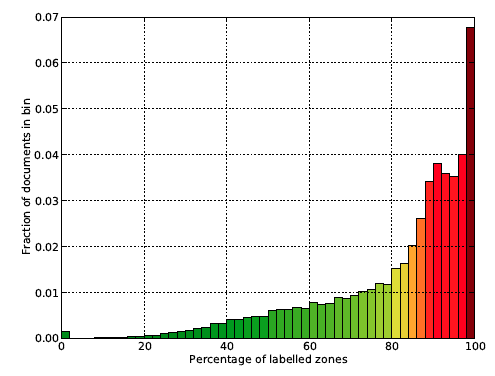
\includegraphics[width=12cm]{plots/zone_coverage_grotoap2}
  \caption{The histogram presents distribution of succesful zone coverage after mapping NLM metadata to PDF files in the Open Access Subset of PubMed. Coverage different than 100\% can be caused by imperfect metadata, wrong PDF segmentation or inefficient mapping algorithm. Image source: \cite{DominikaTkaczykPaweSzostek2014}.}
  \label{fig:trueviz_match_histogram}
\end{figure}
\begin{enumerate}
\item NLM files in PMC vary in quality. Those with less detailed metadata resulted in barely labeled TrueViz files,
\item With certain layouts our segmentation algorithm was failing, producing very finely-grained text zones with just a handful of letters each. In these cases it was barely possible to match NLM metadata with the actual text, what again lead to sparsely labeled TrueViz files. 
\end{enumerate}
In order to assure good quality of the final set we needed to filter out documents with TrueViz files of bad quality. In the figure \ref{fig:trueviz_match_histogram} one can see a distribution of documents with a given fraction of labeled zones.
Based on this distribution we decided to keep the documents having at least 90\% of labeled zones.

\section{TrueViz file format} \label{sec:trueviz_file_format}
We decided to choose TrueViz file format as the data set's main data format. This was to maintain the choice taken while working on GROTOAP data set. The motivation behind this choice is discussed in details in \cite{Tkaczyk2012}. TrueViz is a plain text file based on the XML format that holds in an extremely inefficient way the content of a document together with its geometrical properties and classification metadata. An example of a dumb file containing a single character is shown on the listing \ref{lst:trueviz_sample}.
\lstinputlisting[label={lst:trueviz_sample},caption={Sample content of a TrueViz file with one letter of content - \textit{F}},basicstyle=\scriptsize,language=XML,frame=lbtr]{samples/trueviz_sample.xml}
The resulting TrueViz files are obviously much bigger than the input PDF file. This is the price that has to be paid for the readability that it offers.

Each of the text zones in a document is labeled with one out of 22 categories:
\begin{itemize}
    \item \verb+abstract+ - document's abstract,
    \item \verb+acknowledgments+ - acknowledgment for article's funding
    \item \verb+affiliation+ - authors' affiliations,
    \item \verb+author+ - document authors,
    \item \verb+author_title+ - zones containing both document's title and the list of authors; This zone has been introduced, as very often our segmentation algorithm 
    \item \verb+bib_info+ - bibliographic information that was not assigned into any other category, usually concerning the journal issue e.g. journal name, publisher name, volume, DOI,
    \item \verb+body_content+ - the text of the document that did not match any other category,
    \item \verb+conflict_statement+ - conflict statement declaration,
    \item \verb+copyright+ - copyright section,
    \item \verb+correspondence+ - contact information to the article's authors, usually includes e-mail addresses, but physical address is also possible,
    \item \verb+dates+ - dates related to the document life-cycle - reception date, review date, publishing date etc.,
    \item \verb+editor+ - name of document's editor,
    \item \verb+equation+ - mathematical equation,
    \item \verb+figure+ - figure captions and figures elements which are embedded in a PDF as text, e.g. axes labels,
    \item \verb+glossary+ - article's glossary,
    \item \verb+keywords+ - article's keywords,
    \item \verb+page_number+ - page number of the volume;
    \item \verb+references+ - article's references with all the data (titles, names, years) put into one bag,
    \item \verb+table+ - table's content and caption;
    \item \verb+title+ - article's title;
    \item \verb+type+ - the type of the document, usually mentioned on the first page near the title, such as \textit{research paper}, \textit{case study} or \textit{editorial};
    \item \verb+unknown+ - used for the text zones that couldn't be assigned to any other category. This might be because they are very rare or couldn't be matched to any metadata.
\end{itemize}
This list is richer than the set of labels used by CERMINE, as we were not targeting such a fine-grained granularity in the system output. On the other hand, Pubmed XMLs are very rich and contain a huge number of metadata elements. It would be a pity to create a data set which would loose silently these data. This is why we decided to keep extended set of categories in GROTOAP2. In the appendix \ref{app:grotoap2} one can see distributions of these catogories for the chosen documents.

The \verb+acknowledgment+ section has a very similar distribution, \verb+affiliation+ is mostly focused in two or three zones with a pretty short tail, \verb+author+ section has a very narrow distribution with most of the articles having only one such zone. On the contrary, \verb+author_title+ is in most cases represented by 4 or 5 zones. \verb+editor+ is, as expected, in the majority of cases present in only one zone per document. It is interesting to see what is the distribution of \verb+unknown+ zones, i.e. those whose content couldn't be matched with the data from Pubmed XML. The most numerous bins are \verb+1+ and \verb+2+, containing in total more than 12000 documents. This can be seen as an indicator of good quality of the data set.

Figure \ref{fig:label_barplot} shows the fraction of documents in the data set that contain given label. One can see that all the documents contain labels \verb+bib_info+, \verb+body_content+, \verb+references+ and \verb+affiliation+.

Figure \ref{fig:label_count_barplot} shows the total count of labels across all documents (logarithmic scale). One can see that \verb+table+ is the most numerous label, followed by \verb+body_content+. This is caused by inability to cluster very small and distant text zones together, as they usually appear so in the tables embedded in the PDF documents.

Figures \ref{fig:publishers_pieplot} and \ref{fig:journals_pieplot} show the contribution in the data set of the top 15 publishers and top 25 journals respectively. In total there are 208 publishers included and 1170 journals. As expected, the biggest publisher is a medical one (BioMed Central), but the remaining ones might be associated with a general scientific publishing. As different journals are stuck to their layouts, we might be sure that the variety of the layouts in the data set is sufficient to allow good mean performance on unknown articles.

Figures \ref{fig:page_count_histogram} and \ref{fig:publication_year_histogram} show the distribution of number of pages and publication years respectively. The first distribution reaches its maximum at 8 pages, which is a standard in the scientific publishing. The second distribution is focused around the year 2010, but has a tail reaching year 1995. Therefore, we might expect that the classifier trained using this set will show better performance for more recent publications.

%%%%%%%%%%%%%%%%%%%%%%%%%%%%%%%%%%%%%%%%%%%%%%%%

\begin{figure}
\centering
\begin{minipage}[t!]{\linewidth}
  \centerline{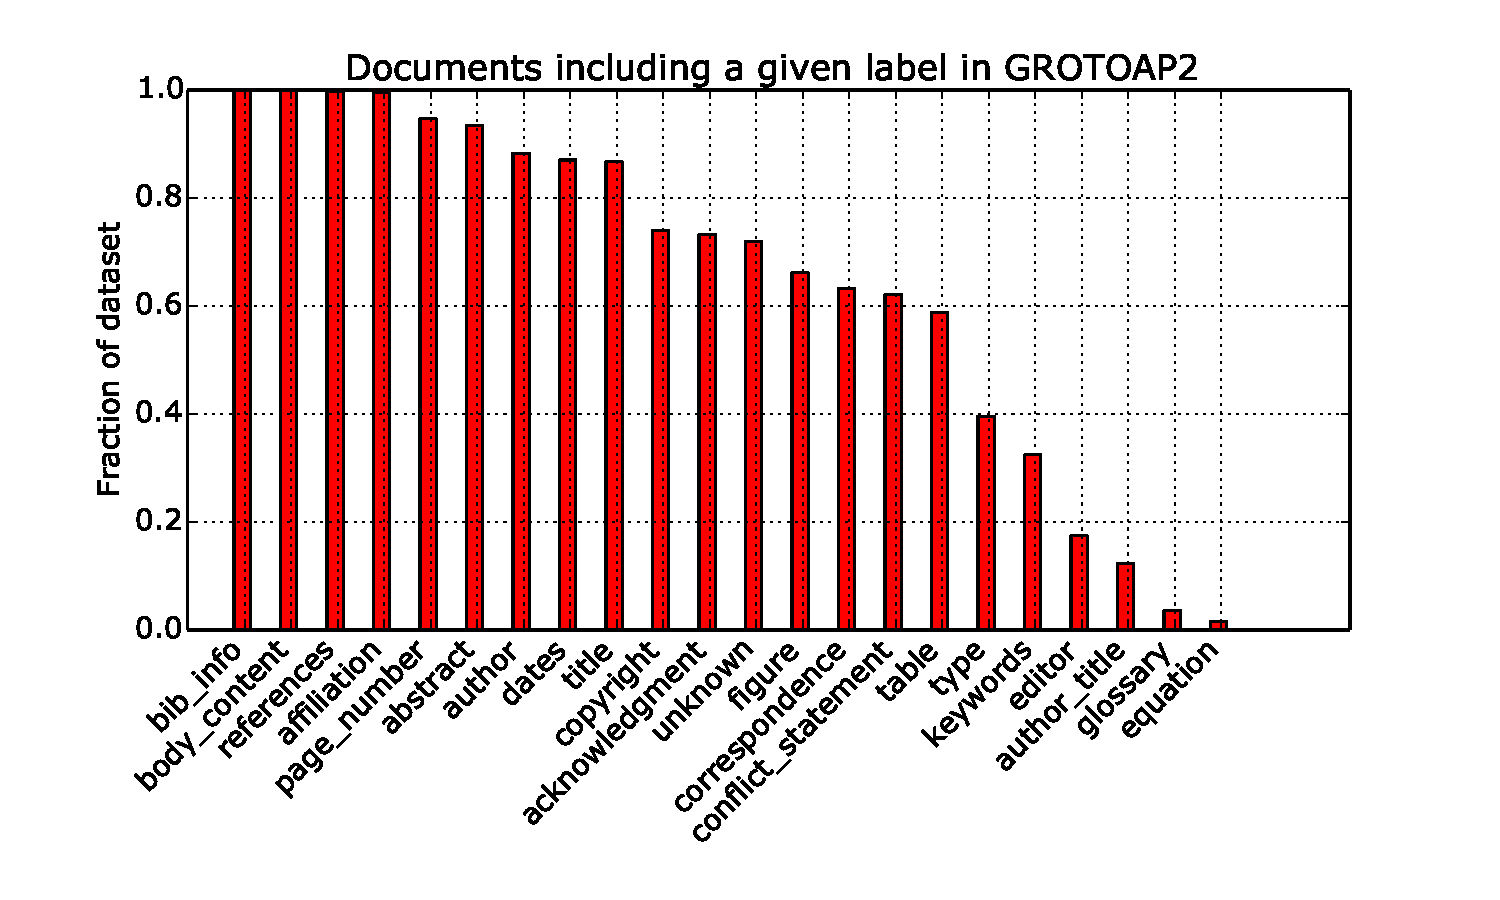
\includegraphics[width=18cm]{plots/docs_with_labels_barplot}}
  \caption{Fraction of documents containing given label}
  \label{fig:label_barplot}
\end{minipage}
\begin{minipage}[t!]{\linewidth}
  \centerline{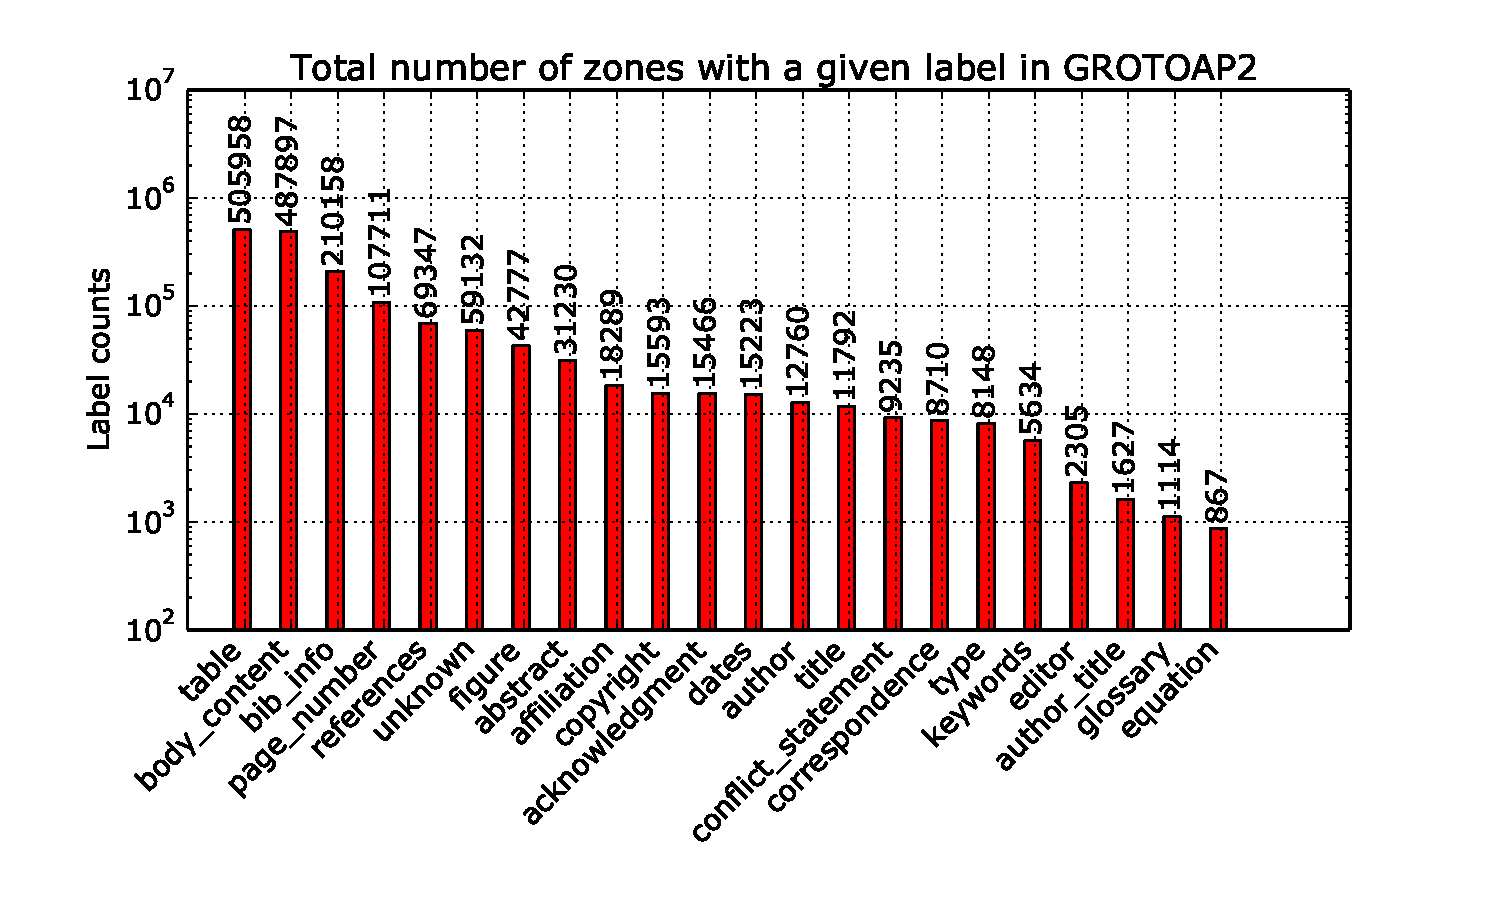
\includegraphics[width=18cm]{plots/label_barplot}}
  \caption{Total count of zones labeled with given label in GROTOAP2}
  \label{fig:label_count_barplot}
\end{minipage}
\end{figure}

  \begin{figure}
  \centering
\begin{minipage}[t!]{\linewidth}
  \centerline{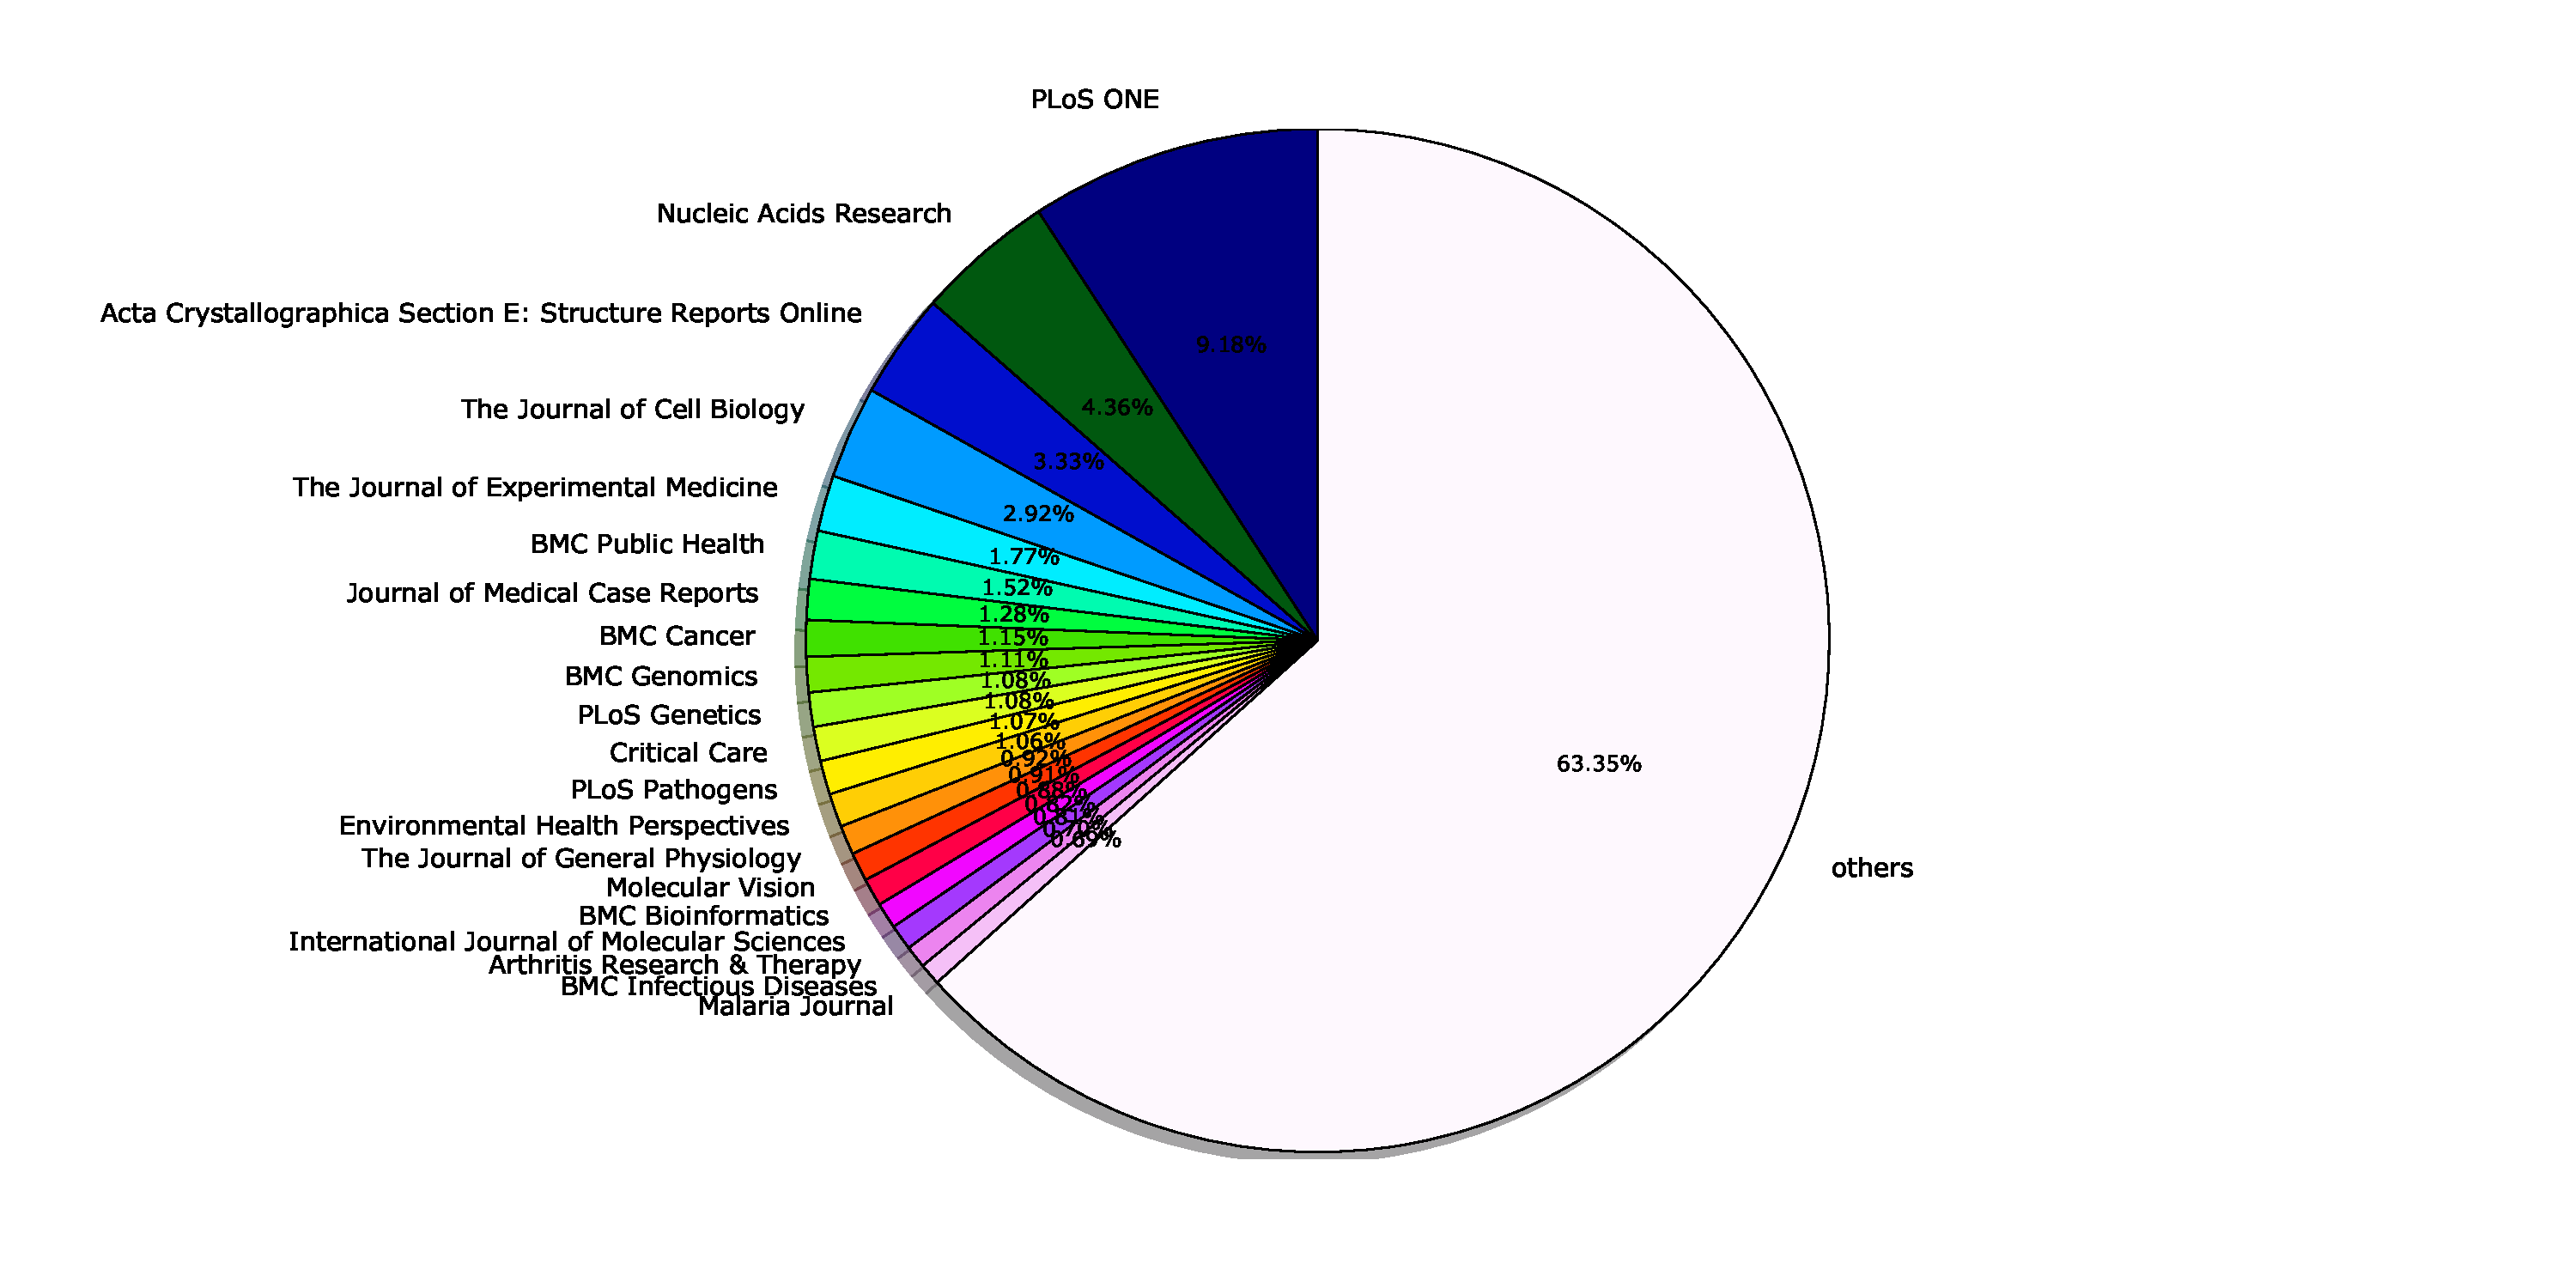
\includegraphics[width=22cm]{plots/journals_pieplot}}
  \caption{Top 25 journals in the GROTOAP2 dataset}
  \label{fig:journals_pieplot}
\end{minipage}
\quad
\begin{minipage}[t!]{\linewidth}
  \centerline{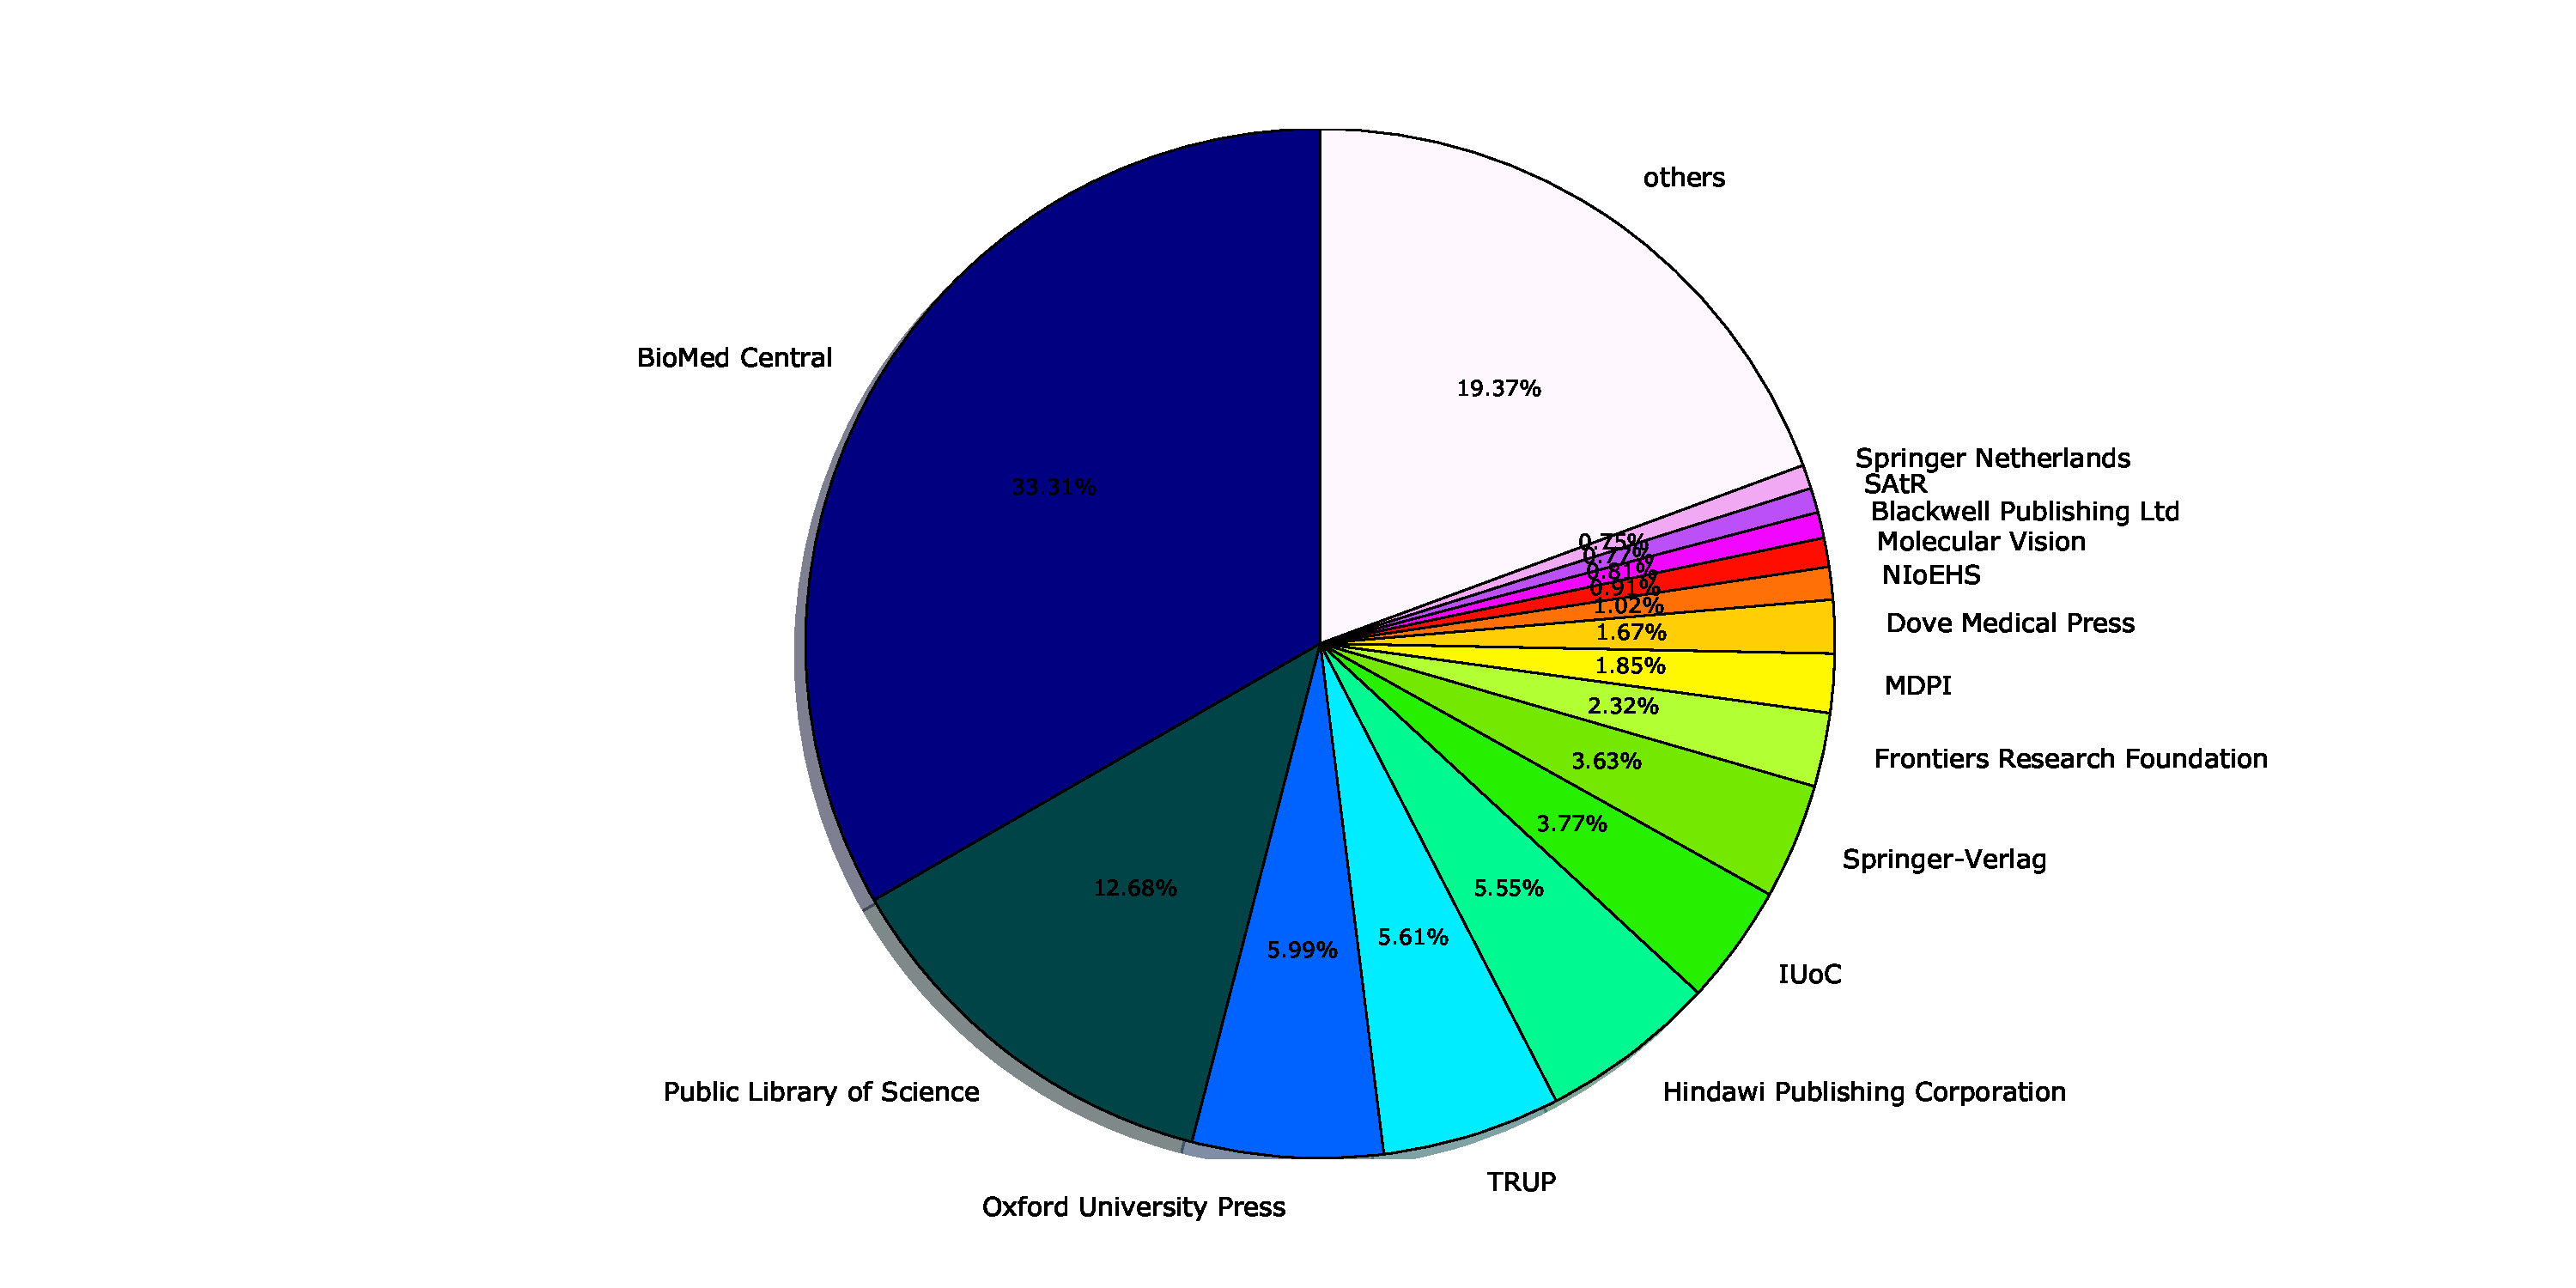
\includegraphics[width=22cm]{plots/publishers_pieplot}}
  \caption{Top 15 publishers in the GROTOAP2 dataset}
  \label{fig:publishers_pieplot}
\end{minipage}
\end{figure}
%%%%%%%%%%%%%%%%%%%%%%%%%%%%%%%%%%%%%%%%%%%

\begin{figure}
  \centering
\begin{minipage}[t!]{0.45\linewidth}
  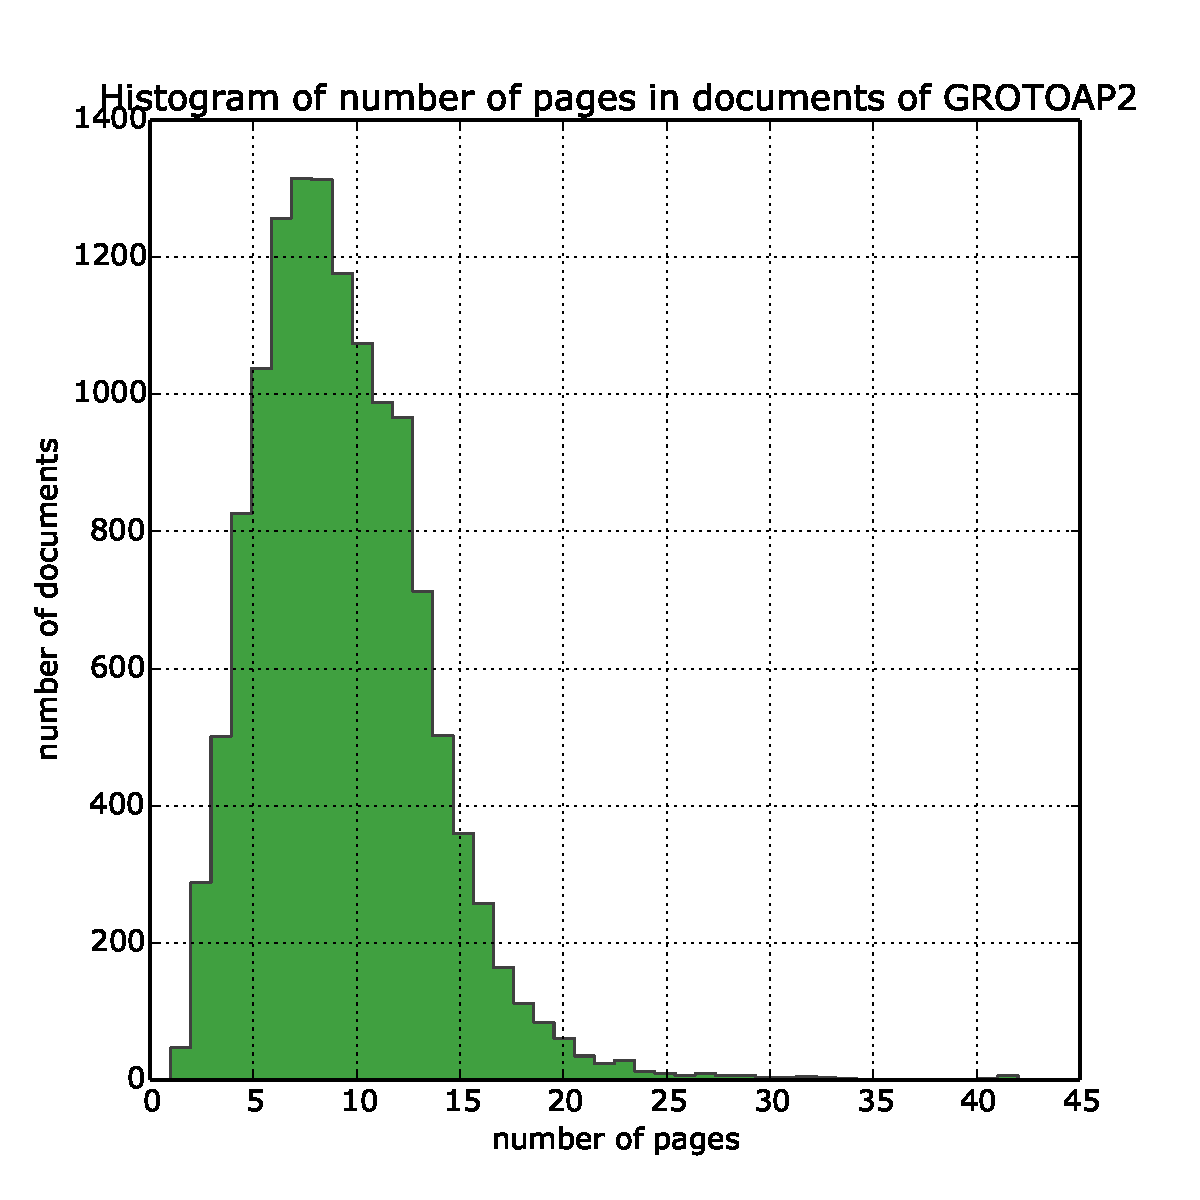
\includegraphics[width=8cm]{plots/pages_histogram}
  \caption{Histogram of number of pages of the documents in the GROTOAP2 dataset}
  \label{fig:page_count_histogram}
\end{minipage}
\quad
\begin{minipage}[t!]{0.45\linewidth}
  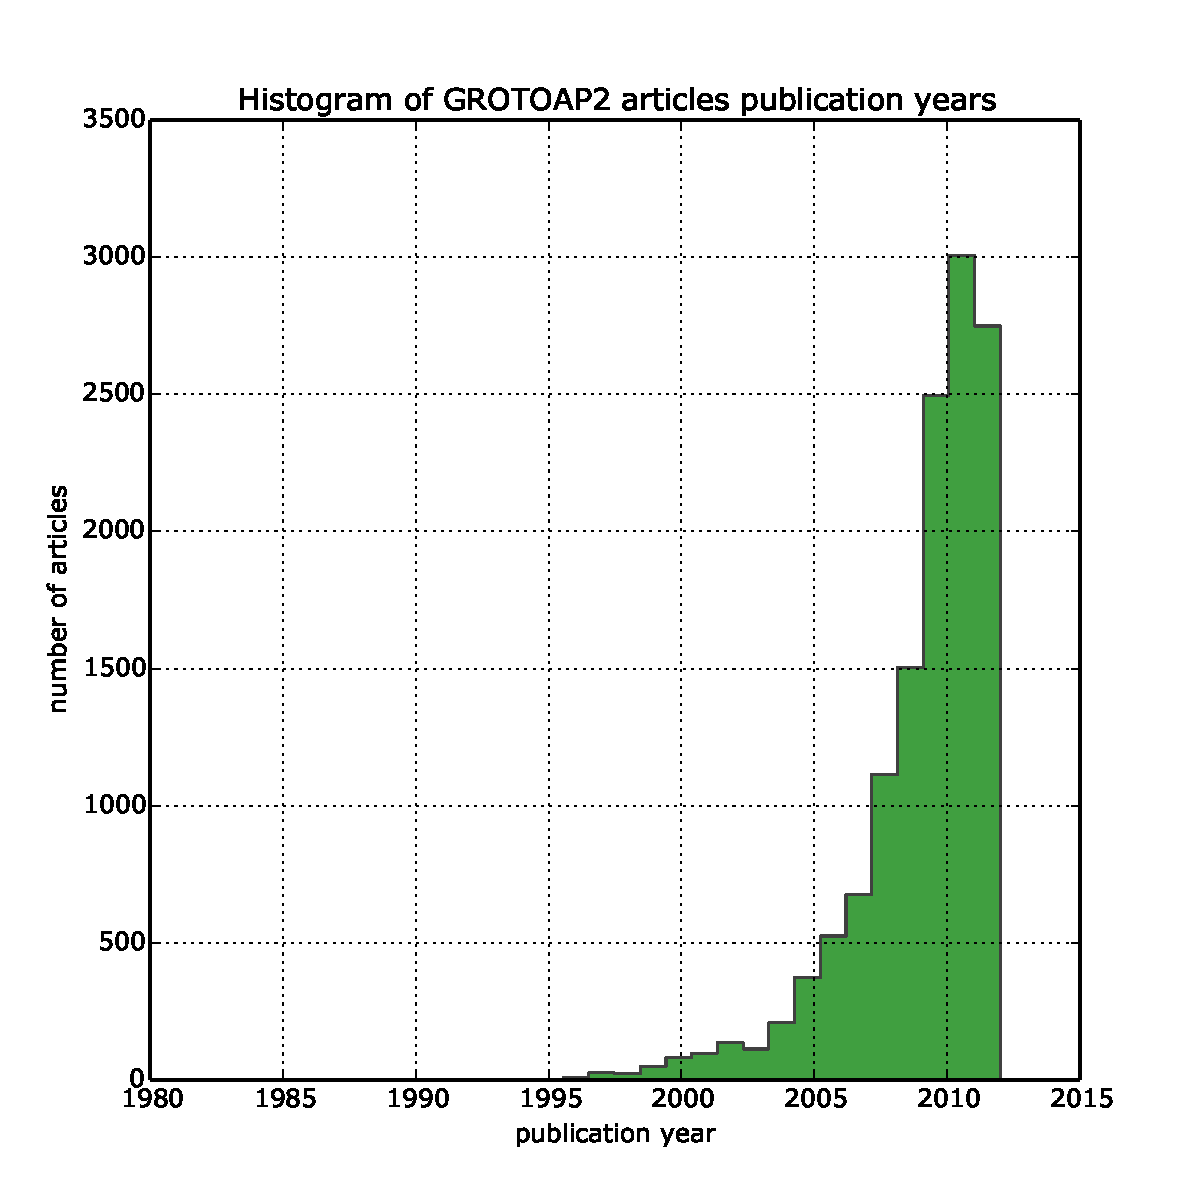
\includegraphics[width=8cm]{plots/publication_year_histogram}
  \caption{Histogram of publication year of the documents in the GROTOAP2 dataset}
  \label{fig:publication_year_histogram}
\end{minipage}
\end{figure}

\section{Dataset evaluation}
Evaluation of the created dataset is precisely described in \cite{DominikaTkaczykPaweSzostek2014}. Evaluation was not done by the author of this thesis. It was entirely performed by author's team mates from the Interdisciplinary Center for Mathematical and Computation Modeling. Nevertheless, its results and methodology will be quoted here in order to make the description more complete.

\quad
For the purpose of evaluation there was a handful of 50 documents picked. Those documents were automatically labeled and then errors were rectified. Subsequently, the corrected documents and the original ones were compared and the factors of precision and recall were calculated. Table \ref{tab:grotoap2_evaluation} shows the values obtained for each label.

\begin{table*}
%\ra{1.3}
\centering
\begin{tabular}{@{}rrrcrrr@{}}
 \toprule
label & precision & recall & \phantom{abc} & label & precision & recall\\ \midrule
abstract & 0.98 & 0.98 && equation & - & - \\ 
acknowledgment & 1.00 & 0.90 && figure & 0.99 & 0.46 \\ 
affiliation & 0.95 & 0.95 && glossary & 1.00 & 1.00 \\ 
author & 1.00 & 0.98 && keywords & 1.00 & 0.94 \\ 
author\_title & 1.00 & 1.00 && page\_number & 0.98 & 0.97 \\ 
bib\_info & 0.96 & 0.94 && references & 0.99 & 0.95 \\ 
body & 0.88 & 0.99 && table & 0.98 & 0.96 \\ 
conflict\_statement & 0.82 & 0.89 && title & 1.00 & 1.00 \\ 
copyright & 0.93 & 0.78 && type & 0.89 & 0.47 \\ 
correspondence & 1.00 & 0.97 && unknown & 0.62 & 0.94 \\ 
dates & 0.94 & 1.00 && * & 0.95 & 0.91 \\ 
editor & 1.00 & 1.00 &&   &      &       \\
\bottomrule
\end{tabular}
\caption{Evaluation metrics for the GROTOAP2 zone labeling process. The automatically generated metrics were manually compared with the actual labels on a subset of GROTOAP2. For each class precision and recall were calculated. Source: \cite{DominikaTkaczykPaweSzostek2014}}
\label{tab:grotoap2_evaluation}
\end{table*}

Another evaluation of the dataset was done by comparing CERMINE performance in two scenarios: trained with GROTOAP and a random handful of 1000 documents from GROTOAP2. Test documents were randomly selected from the Pubmed Central collection. Table \ref{tab:grotoap2_cermine_evaluation} shows results of the evaluation. One can notice that the F-score of classifier based on GROTOAP2 has grown by 16.93\%.

\begin{table*}[]
\centering
\begin{tabular}{@{}rrr@{}}
\toprule
& GROTOAP & GROTOAP2 \\
\midrule
precision & 77.13\% & 82.22\% \\
recall & 55.99\% & 76.96\% \\
F-score & 62.41\% & 79.34\% \\
\bottomrule
\end{tabular}
\caption{Evaluation of GROTOAP2 using CERMINE trained with GROTOAP and GROTOAP2.}
\label{tab:grotoap2_cermine_evaluation}
\end{table*}

